The Bayesian framework discussed in \cref{sec:ICASP:Networks} is now applied to analyze the experimental data that was presented in \cref{sec:ICASP:Data}.
% KNOWN HYPERPARAMETERS
More specifically we use the first two batches of experiments that were conducted in 2009 and 2010 to calibrate the unknown coefficients of the model \cref{eq:ICASP:Known:BPN}.
For those batches the amount of component-level data is deemed sufficient to fit the hyperparameters and to treat them as knowns subsequently.
% UNKNOWN HYPERPARAMETER
Moreover the first four batches will be analyzed with the model \cref{eq:ICASP:Unknown:BPN} that allows to treat the hyperparameters as unknowns.
Especially in the years 2011 and 2012 the small amount of component-level data does not allow to proceed in another way.
% VALIDATION SET
The fifth batch of experiments from 2014 will be used as an independent test set.
\par % PRIOR ELICITATION
Since the coefficients in \cref{eq:ICASP:ProbabilisticInterpretation,eq:ICASP:AleatoryUncertainty} cannot be identified with those of \cref{eq:ICASP:EmpiricalRelation},
it is not possible to elicit informative priors about the former by exploiting expert knowledge or code information about the latter.
Hence uninformative priors are used.
Specifically we assign uniform prior distributions \(\pi(k) = \mathcal{U}(0,1)\) and \(\pi(\alpha) = \mathcal{U}(0.5,1)\).
Due to \(\beta=1-\alpha\) the latter assignment enforces \(\alpha \geq \beta\).
This reflects the intuition that, regarding the masonry compressive strength, the brick units are more influential than the mortar.
% HYPERPRIOR ELICITIATION
For the Bayesian model in \cref{eq:ICASP:Unknown:BPN} priors \(\pi(\bm{\theta}_{b,i}) = \pi(\mu_{b,i}) \, \pi(\sigma_{b,i})\) and \(\pi(\bm{\theta}_{m,i}) = \pi(\mu_{b,i}) \, \pi(\sigma_{b,i})\)
have to be elicited for the unknown hyperparameters.
We use independent uniform hyperprior distributions with reasonable bounds for the means and standard deviations.
\par % POSTERIORS
The posteriors \cref{eq:ICASP:Known:Posterior,eq:ICASP:Unknown:Posterior} can be sampled by means of Markov chain Monte Carlo (MCMC) techniques \cite{MCMC:Brooks2011}.
In \cref{fig:ICASP:Post:k,fig:ICASP:Post:alpha} the resulting posterior marginals of \(k\) and \(\alpha\) are depicted.
% COMPARISON: KNOWN / UNKNOWN
It can be seen that \(\pi(k,\alpha \cond \tuple{f_{w,ij}},\tuple{f_{b,ik}},\tuple{f_{m,il}})\) contains a higher degree of posterior uncertainty than \(\pi(k,\alpha \cond \tuple{f_{w,ij}})\).
Since more data has entered the former posterior, at first sight this seems to be surprising.
This fact can be attributed to the differences of the models \cref{eq:ICASP:Known:BPN,eq:ICASP:Unknown:BPN} in treating the hyperparameters and their uncertainties, though.
% POSTERIOR: k
\begin{figure}[ht]
  \centering
  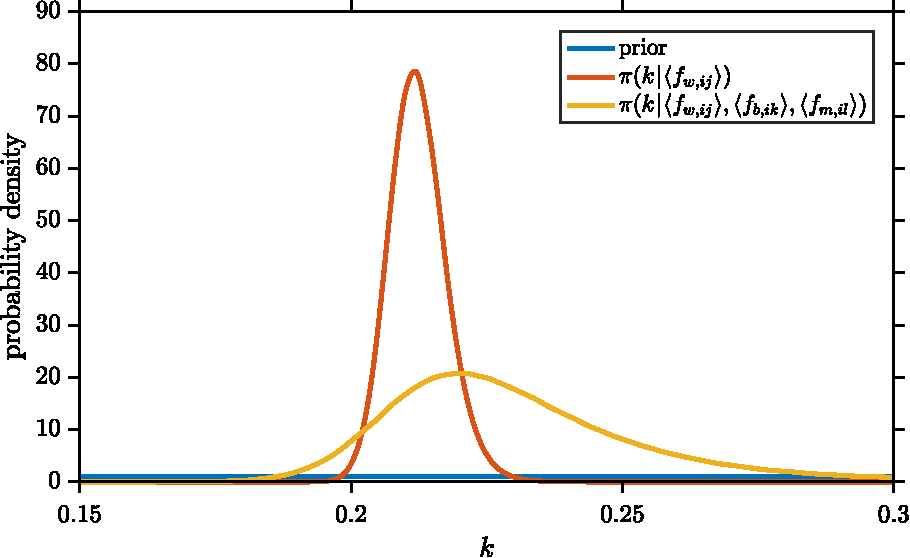
\includegraphics[width=\ICASPfigWidth]{fig_ICASP_Post_k}
  \caption[Posterior of \(k\)]{Posterior of \(k\).
           The posteriors \(\pi(k \cond \tuple{f_{w,ij}})\) and \(\pi(k \cond \tuple{f_{w,ij}},\tuple{f_{b,ik}},\tuple{f_{m,il}})\) are shown.
           It can be seen that the latter is broader than the former.
          }
  \label{fig:ICASP:Post:k}
\end{figure}
% POSTERIOR: alpha
\begin{figure}[ht]
  \centering
  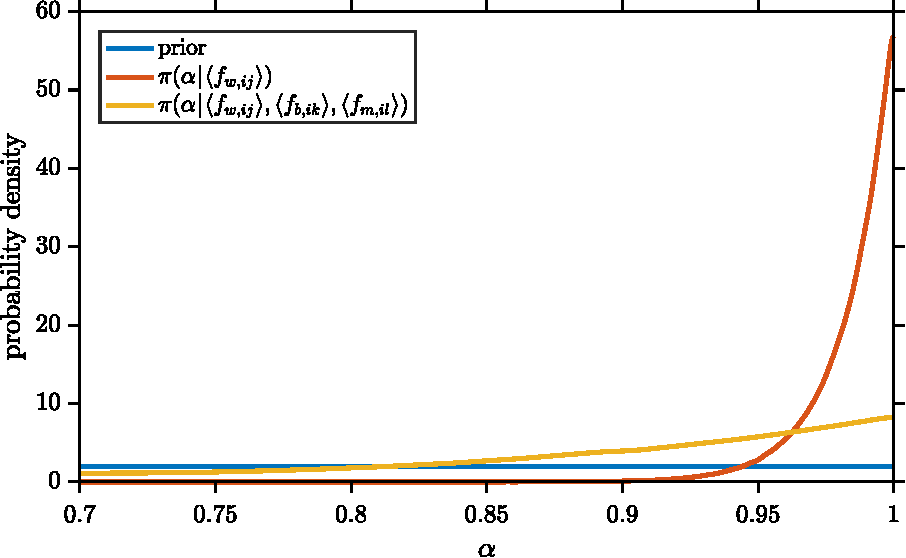
\includegraphics[width=\ICASPfigWidth]{fig_ICASP_Post_alpha}
  \caption[Posterior of \(\alpha\)]{Posterior of \(\alpha\).
           Both the posterior marginals \(\pi(\alpha \cond \tuple{f_{w,ij}})\) and \(\pi(\alpha \cond \tuple{f_{w,ij}},\tuple{f_{b,ik}},\tuple{f_{m,il}})\) peak at their upper boundary.
          }
  \label{fig:ICASP:Post:alpha}
\end{figure}
\par % COMPARISON: POSTERIOR MODES: K / ALPHA
Specifically the modes \(\hat{k} = 0.21\) and \(\hat{\alpha} = 1\) are found for the posterior \(\pi(k,\alpha \cond \tuple{f_{w,ij}})\) that represents the situation that hyperparameters are assumed to be known.
The posterior \(\pi(k,\alpha \cond \tuple{f_{w,ij}},\tuple{f_{b,ik}},\tuple{f_{m,il}})\), for the scenario that hyperparameters are treated as unknowns, features the modes \(\hat{k} = 0.22\) and \(\hat{\alpha} = 1\).
\par % PEAK AT THE BOUND
The fact that the posterior of \(\alpha\) in \cref{fig:ICASP:Post:alpha} peaks at the upper bound of its prior is somewhat surprising.
% NEGLIGIBLE MORTAR
As a consequence of \(\hat{\beta} = 1-\hat{\alpha} = 0\), the influence of mortar occurs to be negligible.
Moreover, such a behavior may indicate that the inverse problem is improperly solved, e.g.\ the true parameter value was accidentally excluded a priori.
% INDEPENDENT ALPHA, BETA
It was therefore tried to relax the assumption \(\beta = 1-\alpha\) by permitting arbitrary values \(\alpha>0\) and \(\beta>0\).
To that end independent priors \(\pi(\alpha)\) and \(\pi(\beta)\) were assigned.
We had to conclude that the limited amount of available data is not sufficiently informative in order to calibrate this extended model.
\par % PREDICTIVE DISTRIBUTION
Plugging the point estimates \(\hat{k}\) and \(\hat{\alpha}\) in \cref{eq:ICASP:AleatoryUncertainty} establishes a predictive relation of the frequency distribution of structural masonry.
For that purpose one has to specify the values or estimates of the hyperparameters \(\bm{\theta}_b\) and \(\bm{\theta}_m\) for the ensembles of bricks and mortar used in the construction of the masonry wall.
The predicted distributions, that are obtained this way for the actually analyzed batches of experiments, describe the masonry wall resistances adequately well.
Since the estimations of the coefficients were informed by the very same data, this does not seem to be very surprising.
Yet this signifies that the representation \cref{eq:ICASP:AleatoryUncertainty} is adjustable enough to match the data.
In turn this may indicate that \cref{eq:ICASP:AleatoryUncertainty} is indeed a suitable representation of the masonry wall compressive strength.
\par % TEST SET
When applied to the fifth batch of experiments the procedure described above can serve as a validation test, i.e.\ the data collected in 2014 are used as an independent test set.
In \cref{fig:ICASP:MeasVsPred:2014} the measured masonry wall compressive strengths are shown together with the their predicted distribution.
The plot is supplemented with the corresponding \(\unit[5]{\%}\)-quantile.
Here the point estimates \(\hat{k}=0.22\) and \(\hat{\alpha}=1\) that were obtained by analyzing the previous four batches are used on one side.
On the other side component-level data \(\tuple{f_{b,5j}}\) and \(\tuple{f_{m,5j}}\) for the fifth batch are used to estimate \(\bm{\theta}_{b,5}\) and \(\bm{\theta}_{m,5}\).
% OBSERVATION
The predictive distribution captures the data fairly well.
Obviously it is of higher quality than the poor code-forecast shown in \cref{fig:ICASP:MeasVsPred:2009}.
% FIGURE: MEASUREMENTS VS. PREDICTIONS
\begin{figure}[ht]
  \centering
  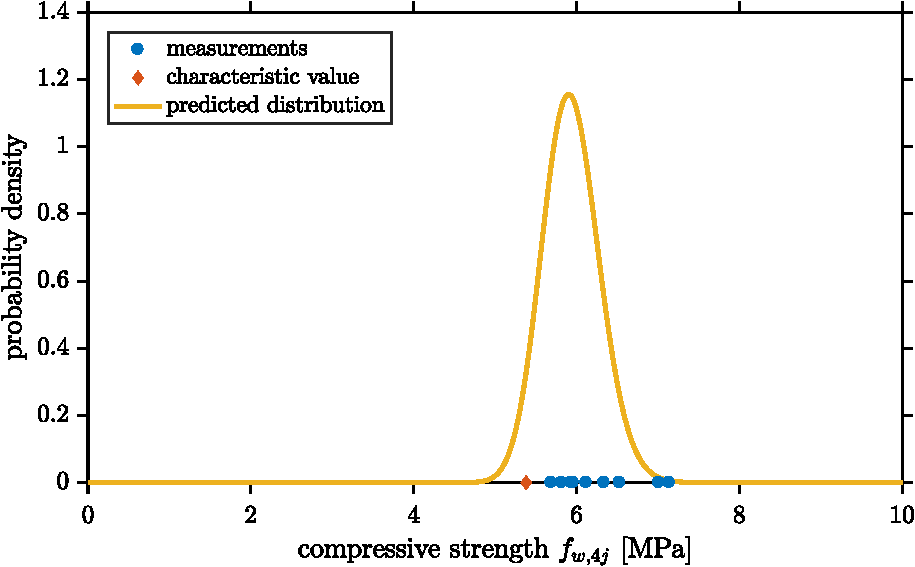
\includegraphics[width=\ICASPfigWidth]{fig_ICASP_PredVsMeas_2014}
  \caption[Data and predictions for 2014]{Data and predictions for 2014.
           The gathered data, the predicted distribution and its \(\unit[5]{\%}\)-quantile are shown.
           Predictions conform to data tolerably well.
          }
  \label{fig:ICASP:MeasVsPred:2014}
\end{figure}